%% qr-front-cover.tex  -*- TeX-master: "qr.tex" -*-

% Copyright (C) 2018 Ralph Schleicher

% Permission is granted to copy, distribute, and/or modify this document
% under the terms of the GNU Free Documentation License, Version 1.3 or
% any later version published by the Free Software Foundation; with no
% Invariant Sections, no Front-Cover Texts, and no Back-Cover Texts.
%
% You should have received a copy of the GNU Free Documentation License
% along with this document.  If not, see <https://www.gnu.org/licenses/>.

%% Code:

\begin{titlepage}
\leavevmode
\vfill

\begin{center}
\usekomafont{disposition}\Huge Quick Reference
\end{center}

\vfill

\begin{center}
\Huge\textsc{pgfplots}
\end{center}

\vskip 4\baselineskip

\begin{quote}
\color{gray}
\begin{verbatim}
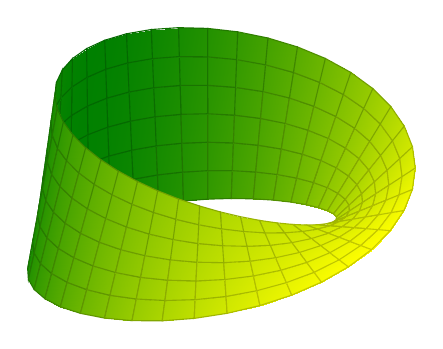
\begin{tikzpicture}
\begin{axis}[
  hide axis,
  view = {40}{40},
]
\addplot3[
  surf,
  colormap/greenyellow,
  shader = faceted interp,
  z buffer = sort,
  point meta = x,
  domain = 0:360,
  domain y = -0.5:0.5,
  samples = 40,
  samples y = 7,
]
({(1 + 0.5 * y * cos(x / 2))) * cos(x)},
 {(1 + 0.5 * y * cos(x / 2))) * sin(x)},
 {0.5 * y * sin(x/2)});
\end{axis}
\end{tikzpicture}
\end{verbatim}
\end{quote}

\vskip 4\baselineskip

% Moebius strip example from <https://pgfplots.net>.
\begin{center}
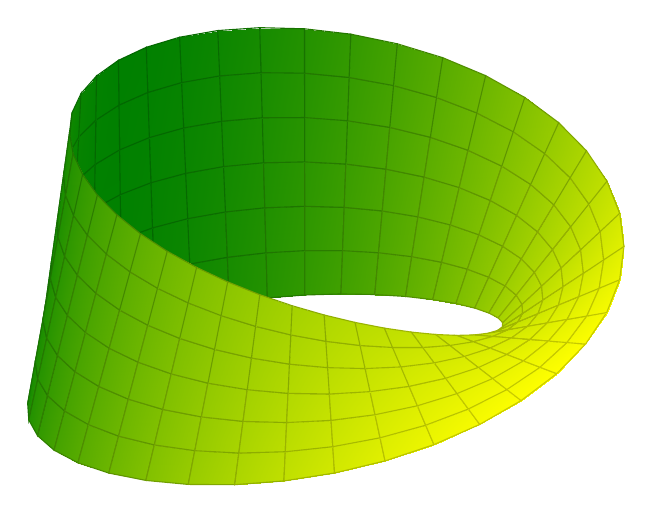
\begin{tikzpicture}
\begin{axis}[
  width=\the\textwidth,
  hide axis,
  view = {40}{40},
]
\addplot3[
  surf,
  colormap/greenyellow,
  shader = faceted interp,
  z buffer = sort,
  point meta = x,
  domain = 0:360,
  domain y = -0.5:0.5,
  samples = 40,
  samples y = 7,
]
({(1 + 0.5 * y * cos(x / 2))) * cos(x)},
 {(1 + 0.5 * y * cos(x / 2))) * sin(x)},
 {0.5 * y * sin(x/2)});
\end{axis}
\end{tikzpicture}
\end{center}

\vskip 4\baselineskip

\begin{quote}
\Large
Ralph Schleicher
\end{quote}

\vfill
\end{titlepage}

%% qr-front-cover.tex ends here
